%\documentclass[12pt,english]{report}
%\usepackage{mathptmx}
%\renewcommand{\familydefault}{\rmdefault}
%\usepackage[T1]{fontenc}
%\usepackage[latin9]{inputenc}
%\usepackage[a4paper]{geometry}
%\setcounter{secnumdepth}{2} % Changed from 3 to 2. 0-chapter 1-section 2-subsection 
%\setcounter{tocdepth}{2} % Changed from 3 to 2. 0-chapter 1-section 2-subsection 
%\setlength{\parskip}{\medskipamount}
%\setlength{\parindent}{0pt}
%\usepackage{verbatim}
%\usepackage{pdfpages}
%\usepackage{graphicx}
%\usepackage{subfig} %% This package has to be here
%\usepackage{setspace}
%\usepackage{arabtex}
%\usepackage[numbers]{natbib}
%\usepackage{nomencl}
%\usepackage{paralist}
%\usepackage{amsthm}
%\usepackage{amsmath}
%\usepackage{amsfonts}
%\usepackage{etoolbox}
%\newtoggle{edit-mode}
%\togglefalse{edit-mode}  
%\toggletrue{edit-mode}
%\iftoggle{edit-mode}{
%\geometry{verbose,tmargin=2cm,bmargin=2cm,lmargin=2cm,rmargin=6cm,headheight=1cm,headsep=1cm,footskip=1cm, marginparwidth=5cm}
%}{
%\geometry{verbose,tmargin=2cm,bmargin=2cm,lmargin=2cm,rmargin=2cm,headheight=1cm,headsep=1cm,footskip=1cm}
%}
%
%\makenomenclature
%
% %Theorem Styles
%\newtheorem{theorem}{Theorem}[section]
% %Definition Styles
%\theoremstyle{definition}
%\newtheorem{definition}{Definition}[section]
%\newtheorem{example}{Example}[section]
%\theoremstyle{remark}
%\newtheorem{remark}{Remark}
%
%\usepackage[linesnumbered]{algorithm2e}
%
%\begin{document}
%
%\tableofcontents{}

%%%%%%%%%%% nomenclature %%%%%%%%%%
\nomenclature{SC}{Shape Context}
\nomenclature{MAD}{Multi Angular Descriptor}
\nomenclature{PCA}{Principal Component Analysis}
\nomenclature{LDA}{Linear Discriminant Analysis}
\nomenclature{DTW}{Dynamic Time Warping}
\nomenclature{EMD}{Earth Mover's Distance}
\nomenclature{LSH}{Locality Sensitive Hashing}
%%%%%%%%%%%%%%%%%%%%%%%%%%%%%%%%%%%%


\chapter{Fast Classification of On-line Handwritten Arabic Characters}
\label{chap:characters_classification}

\iftoggle{edit-mode}{\hspace{0pt}\marginpar{The learning process}}{}
Letter samples extracted from the ADAB databases were split into four groups according to their position: \textbf{Ini}, \textbf{Med}, \textbf{Fin} and \textbf{Iso}. 
The set of samples in each position undergone a learning process that contains five main stages.
First, the samples were preprocessed as described in Section \ref{sec:preprocessing}.
Second, feature vectors were extracted as detailed in Section \ref{sec:feature_extraction}.
Then, the feature vectors were embedded into the $L_1$ metric space by extracting the scaled coefficients of the wavelet transformation, as presented in Section \ref{sec:similarity_search}.
This was done to enable fast computation of intuitive similarity search techniques, described in Section \ref{sec:similarity_measures}.
In Section \ref{sec:dr}, we outline a dimensionality reduction process that obtains a compact representation of the high dimensional vectors produced by the embedding procedure.
In the last stage, described in Section \ref{sec:metric_indexing}, we build a metric index that enables finding the most similar object in sub-linear time.

\iftoggle{edit-mode}{\hspace{0pt}\marginpar{The recognition process}}{}
The classification process corresponds to the learning process.
Given an un-labelled query sequence, the sequence undergoes preprocessing, features extraction, embedding and dimensionality reduction.
The low dimensional vector is then used to to find the closest ten sample among the large list of sample containing more than a thousand instances.
As described in Section \ref{sec:candidates_scoring}, we then allow the usage of an accurate and expensive similarity measure technique to rank the short list of candidates. \\
An overview of the learning and classification processes is given in Figure \ref{fig:classification_system_flow}.

\begin{figure}
\centering
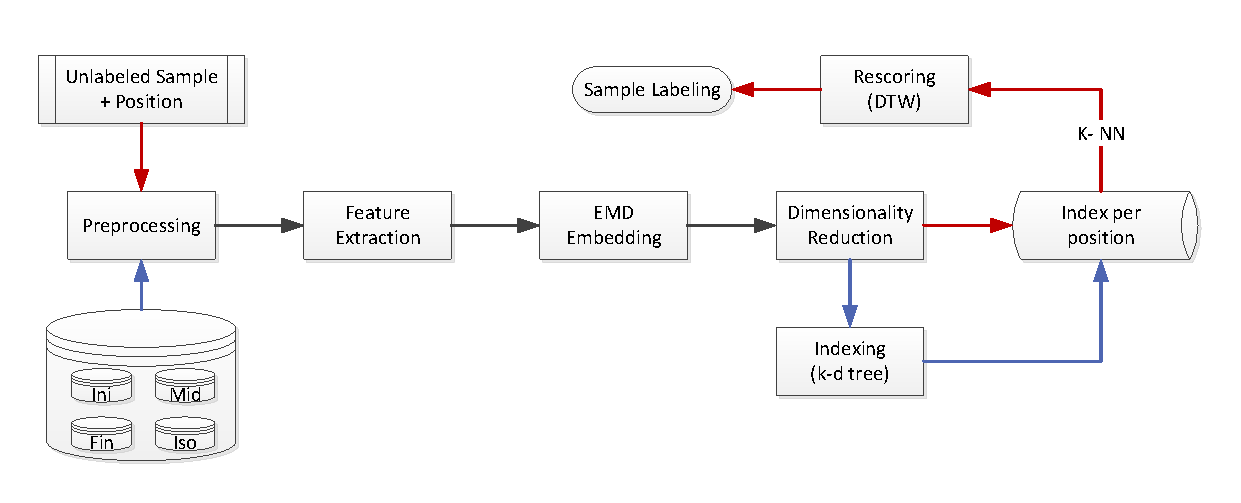
\includegraphics[width=1\textwidth]{./figures/classification_system_flow}
\caption{High level diagram of both the training and classification flows. The blue arrows indicate parts that are unique to the training process and the red arrows indicate parts that are unique to the classification process.}
\label{fig:classification_system_flow}
\end{figure}


%Thus a re-scoring stage using a costly but accurate similarity measure is applied on a short list of candidates.   
%The scoring of candidates based on the approximate EMD metric may not sufficiently precise for application that use the this scoring to perform delicate analysis tasks, such as the recognition-based segmentation approach described in Chapter \ref{chap:strokes_segmentation}.

%%%%%%%%%%%%%%%%%%%%%%%%%%%%%%%%%%%%%%%%%%%%%%%%%%%%%%%
\newpage{}
%%%%%%%%%%%%%%%%%%%%%%%%%%%%%%%%%%%%%%%%%%%%%%%%%%%%%%%

\section{Samples Preprocessing}
\label{sec:preprocessing}

\iftoggle{edit-mode}{\hspace{0pt}\marginpar{Introduction}}{}
Digitizers tend to generate a jagged and non-uniform sampling of the trajectory scribed on their surface.
Such devices, normally, sample the input in constant time intervals, thus, slow pen motion regions are over-sampled and fast motion regions are under-sampled.
Further imperfections are caused by hand vibrations resulting from hesitant writing \cite{huang2009preprocessing}.
This lack of uniformity in the data, if not deliberately used by the classification system, should be reduced to avoid negative influence the classification system performance.
In order to overcome the flaws mentioned, preprocessing operations are usually needed to impose certain uniform structure on the data, to comply with the input structure required for the proper operation of the subsequent parts of the system \cite{al2011online}.

\iftoggle{edit-mode}{\hspace{0pt}\marginpar{Preprocessing steps usage}}{}
In the current work, preprocessing consists of three methods: \textbf{normalization}, \textbf{noise elimination} and then \textbf{re-sampling}.
While these three techniques were applied in the mentioned order in both learning and classification of letters, these steps were selectively activated in the segmentation system according to the needs of the specific step.
Other less commonly used preprocessing steps in the field of on-line Arabic HWR, such as rotation and slant normalization \cite{jaeger2001online}, were not implemented in this work. 


\subsection{Normalization}
\iftoggle{edit-mode}{\hspace{0pt}\marginpar{Goal}}{}
Size normalization is performed to achieve a uniform size of the bounding box surrounding the pattern. 
It was applied on each sequence so that it will fit into a $[0,1]\times[0,1]$ bounding box without affecting the original aspect ratio. 
This stage includes an additional step of translating the sequence so that the sequence's center of gravity is located in the origin point, i.e., at $[0,0]$.
Although the features used in this work are agnostic to the pattern's size and location, this step is mostly required by the segmentation flow.

\iftoggle{edit-mode}{\hspace{0pt}\marginpar{Approach}}{}
Given the stroke sequence $S=\{p_i\}_{i=1}^{n}=\{(x_i,y_i)\}_{i=1}^{n}$, the normalized sequence $\bar{S}=\{\bar p_i \}_{i=1}^{n}=\{(\bar x_i,\bar y_i)\}_{i=1}^{n}$ is calculated by: 
\begin{equation}
{\bar x_i} = {{\left( {{x_i} - {\mu _x}} \right)} \over W},{\bar y_i} = {{\left( {{y_i} - {\mu _y}} \right)} \over W}
\end{equation}
where $W = \max (d_x,d_y)$, $d_x$ and $d_y$ are the width and hight of the sequence, respectively, and $\mu$ is the center of gravity of the it, i.e., 
\begin{equation}
\mu  = \left( {{\mu _x},{\mu _y}} \right) = \left( {{1 \over N}\sum\limits_{i = 1}^N {{x_i}} ,{1 \over N}\sum\limits_{i = 1}^N {{y_i}} } \right)
\end{equation}


\subsection{Noise Elimination}

\iftoggle{edit-mode}{\hspace{0pt}\marginpar{Introduction}}{}
The input obtained by the digitizer usually contains a large amount of noise irrelevant for pattern classification. 
This noise consists mainly of redundant points duplication and inadequacies caused by hand vibrations. 
The \emph{Douglas-Peucker Polyline Simplification} algorithm described in \cite{douglas1973algorithms}, also known as the \emph{Iterative Endpoint Fit} algorithm, was used for eliminating such deficiencies in the data. 

\iftoggle{edit-mode}{\hspace{0pt}\marginpar{The Douglas-Peucker algorithm}}{}
The algorithm reduces the number of vertices in a piecewise linear curve, given a pre-set tolerance parameter $\varepsilon$, which defines the maximum 'dissimilarity' between the original and the reduced curve.
It outputs a simplified curve, that consists of a subset of the points in the original curve.
The algorithm operates as follows. 
Initially, it marks the first and the last points to be kept, then it finds the furthest point, $p$, from the line segmented with the first and last points as end points.
If the distance is smaller that $\varepsilon$, the algorithm returns. 
Otherwise, $p$ is kept, and the algorithm recursively operates on the the first point and $p$ and then with $p$ and the last point.
When the recursion is completed, the kept points define an angular skeletonization of the original curve.

\iftoggle{edit-mode}{\hspace{0pt}\marginpar{Different tolerance parameters}}{}
In the normal preprocessing flow, in which normalization is done prior to the simplification process, we empirically set $\varepsilon  = {1 \over 75}$.
However, in cases where normalization is not applicable, such as in the segmentation system, the tolerance parameter has to be dependent on the the pattern's un-normalized bounding box area. 
In such cases, the tolerance parameter was set to: $\varepsilon  = {1 \over {200}}\sqrt {{d_x}^2 + {d_y}^2}$, where $d_x$ and $d_y$ are the width and height of the pattern, respectively. 
The division factors of both cases were tuned empirically. 
The discrepancy in the division factors can be explained by the difference in the sensitivity required in the two flows. 

\subsection{Re-sampling}
\iftoggle{edit-mode}{\hspace{0pt}\marginpar{Goal}}{}
The simplification process produces a highly angular, and non-uniform distribution of points along the stroke trajectory.
Naturally, there are less points in straight areas and a higher density of points in the curved areas stroke. 
This stage, using splines interpolation method, we produce an equidistant smoothed data sequence for a given re-sampling target number of points, $R$. 

\iftoggle{edit-mode}{\hspace{0pt}\marginpar{Approach}}{}
Given a stroke $S=\{(x_i,y_i)\}_{i=1}^{n}$, let $f_{x}(d)$ and $f_{y}(d)$ be the quadratic piecewise interpolations function of $\{x_i\}_{i=1}^{n}$ and $\{y_i\}_{i=1}^{n}$, respectively. 
$f_{x}(d)$ and $f_{y}(d)$ are functions of the coordinate values with respect to the arc-length distance from the pattern's starting point. 
Let $t_i=i\frac{L}{R}$ for $i=0,...,R$ where L is the arc-length of the pattern.
The re-sampled sequence is given as follows:
\begin{equation}
\widehat{S}=\{(f_x(t_i),f_y(t_i))\}_{i=1}^{R}
\end{equation}
Figure \ref{fig:before_after_preprocessing} demonstrates the pre-processing steps applied on a handwritten letter sample.
In our case, we set $R=40$.

\begin{figure}
	\centering
        \subfloat[]{
            \label{fig:preprocessing_orig}
            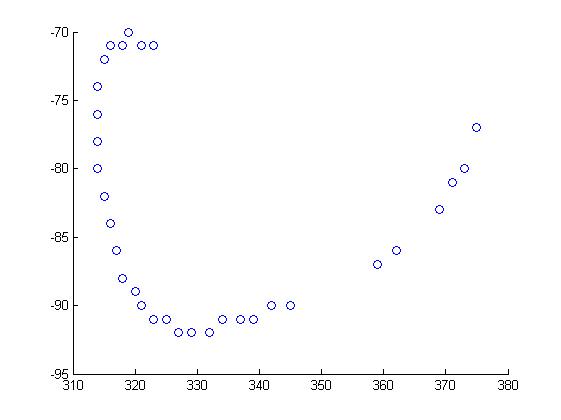
\includegraphics[width=0.4\textwidth]{./figures/preprocessing_orig}
        }
        \subfloat[]{
           \label{fig:preprocessing_norm}
           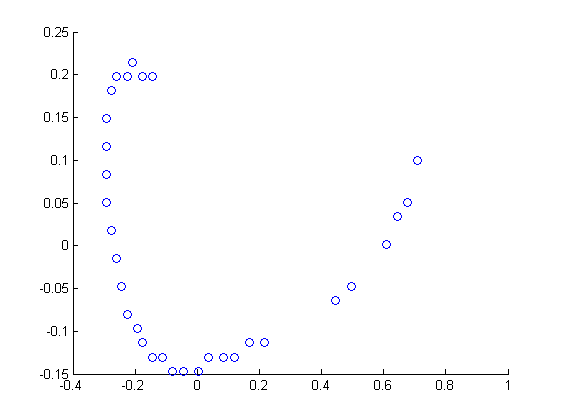
\includegraphics[width=0.4\textwidth]{./figures/preprocessing_norm}
        }  \\
        \subfloat[]{
            \label{fig:preprocessing_simpl}
            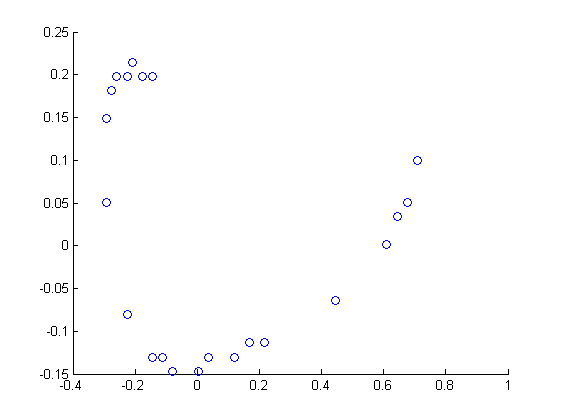
\includegraphics[width=0.4\textwidth]{./figures/preprocessing_simpl}
        }
        \subfloat[]{
           \label{fig:preprocessing_resamp}
           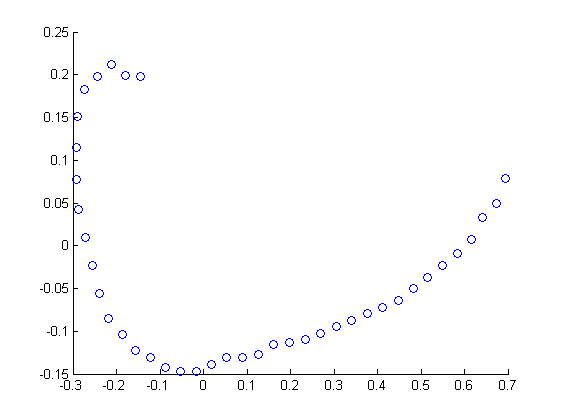
\includegraphics[width=0.4\textwidth]{./figures/preprocessing_resamp}
        }       
    \caption{A sample of the character \RL{b} before preprocessing (\ref{fig:preprocessing_orig}); after normalization (\ref{fig:preprocessing_norm}); after noise elimination (\ref{fig:preprocessing_simpl}) and after re-sampling (\ref{fig:preprocessing_resamp}).}
   \label{fig:before_after_preprocessing}
\end{figure}


%%%%%%%%%%%%%%%%%%%%%%%%%%%%%%%%%%%%%%%%%%%%%%%%%%%%%%%
\newpage{}
%%%%%%%%%%%%%%%%%%%%%%%%%%%%%%%%%%%%%%%%%%%%%%%%%%%%%%%

\section{Shape Descriptors}
\label{sec:feature_extraction}
\iftoggle{edit-mode}{\hspace{0pt}\marginpar{Feature extraction}}{}
Feature extraction is the process of extracting informative parameters for learning and recognition of patterns. 
Poor feature extraction and selection will, in most cases, result in a poor system performance, regardless of the sophistication of the classification algorithm \cite{parizeau2001character}.
The transformation to the feature space is done by extracting descriptive and expressive information from the raw data representation. 
A desired feature extraction technique should facilitate assessing the similarity degree between two objects by maintaining that the distance between them in the feature space reveals their similarity in the real world, and to do so inexpensively.

\iftoggle{edit-mode}{\hspace{0pt}\marginpar{Introduction - Cont.}}{}
In the field of image retrieval and off-line text recognition, the input data is too large and tends to be redundant, thus, feature extraction techniques are used to reduce the representation of the input data. 
However, in the case of recognising on-line handwritten shapes, the input data are compact and feature extraction techniques create feature vector referred to as the \emph{shape descriptor}, which offer discriminative characterization that capture the perceptual dissimilarity between two shapes. 
Unlike the first case in which the features extraction process is a form of data representation reduction, the raw amount of data contained in the shape descriptors usually exceeds the amount of data in the original input data.

\iftoggle{edit-mode}{\hspace{0pt}\marginpar{Shape Descriptors}}{}
Effective shape descriptor must have some essential properties such as invariance under translation, rotation and scale. 
A desirable shape descriptor should have a compact representation and must be easy to compute \cite{zhang2004review}.
It also have to be robust to noise so that distorted shapes which are tolerated by human beings when comparing shapes should be endured also by the shape descriptor \cite{zhang2004review, kim2000region}.

\iftoggle{edit-mode}{\hspace{0pt}\marginpar{Shape descriptors types}}{}
A common classification of shape descriptors is to local and global descriptors. 
Local descriptors calculate a given feature independently at each sample point. 
An example for a simple local feature is the vector containing the tangent slope angle for every given point in the sample point.
Descriptors such as cusps, crossings and loops are referred to as global descriptors and are calculated on the entire shape \cite{hu1997combining}. 
For a comprehensive review on shape descriptors see \cite{zhang2004review} and \cite{yang2008survey}.

\iftoggle{edit-mode}{\hspace{0pt}\marginpar{Using off-line shape descriptors for on-line HWR}}{}
Many of the well known and powerful feature sets operate on the shape's contour.  
However, the input data in the on-line case is a sequence of points representing the pattern trajectory and no contour is involved. 
Using feature sets that were originally developed for contours for recognizing contour-less shapes is common. 
Saabne and El-Sana employed the \emph{Shape Context} (SC) descriptor, a global shape descriptor that was originally developed for contour based shapes, for on-line handwriting recognition in \cite{saabni2009hierarchical}. 
Another example is the usage of the \emph{Multi scale shape context} for on-line handwritten mathematical expressions segmentation in \cite{husegmenting}. \\
In this work we employed and compared two shape descriptors, the SC descriptor and the \emph{Multi Angular Descriptor} (MAD). 

\iftoggle{edit-mode}{\hspace{0pt}\marginpar{Shape Context}}{}
The SC descriptor was presented by Belongie and Malik in \cite{belongie2002shape}.
Given a sequence of points $S=\{p_i\}_{i=1}^n$, the descriptor of the point ${p_i}$, is the coarse histogram of the relative coordinates as defined in Equation \ref{eq:sc_bins}.
The basic idea of the SC descriptor is illustrated in Figure \ref{fig:shape_context_demo}. 
\begin{equation}
{h_i}(k) = \# \{q \ne p_i:(q - p_i) \in bin(k) \}
\label{eq:sc_bins}
\end{equation}
The SC vector of the entire pattern is defined as the concatenation of all the point descriptors.
The bins are normally taken to be uniform log-polar space, making the descriptor more sensitive to positions of nearby sample points than to those of points farther away. 

\begin{figure}
\centering
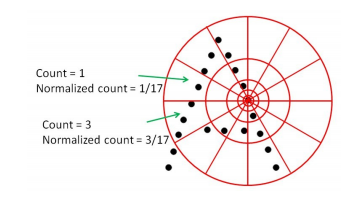
\includegraphics[width=0.3\textwidth]{./figures/shape_context_online}   
\caption{Diagram of the log-polar bins used to compute the Shape Context.}
\label{fig:shape_context_demo}
\end{figure}

\iftoggle{edit-mode}{\hspace{0pt}\marginpar{MAD}}{}
The other shape descriptor used in this thesis is the MAD, which was proposed by Saabne in \cite{saabni2013multi}. 
It captures the angular view from multi resolution rings in different heights. 
The shape is treated as a two dimensional set of points and the different rings are upper view points from rings around the shape centroid with different sizes and heights. 
To enable scale and translation invariance, the sizes and heights of these rings are calculated using the diameter and centroid of the shape.
Formally, let $S$ be a shape and Let $C$ and $D$ be the centroid and the diameter of the shape respectively. 
Let $S = \{p_j\}_{j = 1}^n$ a set of $n$ point taken uniformly on the shape. 
Let $R$ be a ring with the radius $r$ and the center $C$ positioned above the shape $S$ with the height $h$. 
Let $V = \{V_i\}_{i = 1}^\ell$ be a set of $\ell$ viewpoints lying uniformly on the ring $R$ and $\alpha(V_{ij})$ to be the angle between the segment $\overline {{V_i}{p_j}}$ and the plain contains the shape $S$. 
When the parameter $j$ goes over all points in the sequence, we get the vector $Vec_i$ describing the shape from the view point $V_i$.
The descriptor is the concatenation the vectors $V_i$ when the parameter $i$ goes over all viewpoints. 
See illustration in Figure \ref{fig:mad_demo}.

In Section \ref{sec:classification_results} we compare the performance of the above descriptors in our implementation. 

\begin{figure}
\centering
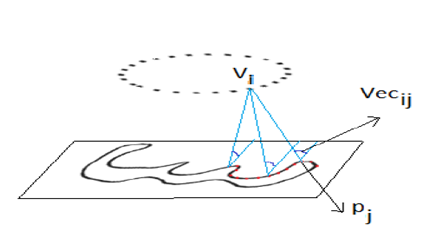
\includegraphics[width=0.5\textwidth]{./figures/mad_demo}       
\caption{A visual demonstration of the Multi Angular Descriptor feature set \cite{saabni2013multi}.}
\label{fig:mad_demo}
\end{figure}

%%%%%%%%%%%%%%%%%%%%%%%%%%%%%%%%%%%%%%%%%%%%%%%%%%%%%%%
\newpage{}
%%%%%%%%%%%%%%%%%%%%%%%%%%%%%%%%%%%%%%%%%%%%%%%%%%%%%%%

\section{Similarity Measures}
\label{sec:similarity_measures}

\iftoggle{edit-mode}{\hspace{0pt}\marginpar{Introduction}}{}
Given two visual data elements, the task of mathematically capturing the human perceptual similarity between them is extremely challenging. 
Similarity measure algorithms aim to quantitatively approximate the perceptual resemblance between data elements. In this chapter, we overview and discuss the different aspects of similarity measure evaluation techniques and present two approaches used in this work.

\iftoggle{edit-mode}{\hspace{0pt}\marginpar{Intuition}}{}
$k$-NN based classification techniques require the ability to correctly and efficiently determine the perceptual distance between two given objects.
Evaluating the dissimilarity between two handwritten strokes based on the raw data representation is difficult and computationally expensive. 
To overcome this hardship, feature extraction methods are used, as described in Section \ref{sec:feature_extraction}, to map the original data into the feature space.  
The similarity measure is formalized as a \emph{distance function}. 
\begin{definition}
Given a data space $\mathfrak{D}$, for any two data elements $x,y \in \mathfrak{D}$, a \textbf{distance function} $dist$, on $\mathfrak{D}$ is defined as:
\begin{equation}
dist: \mathfrak{D} \times \mathfrak{D} \longrightarrow \mathds{R}_{\geq 0} 
\end{equation}
where $dist$ has the following properties:
\begin{compactitem}
\item $dist(x,y)=0 \Leftrightarrow x=y$ (reflexivity)
\item $dist(x,y) = dist(y,x)$ (symmetry)
\end{compactitem}
The pair $(\mathfrak{D},dist)$ is called a \textbf{distance space}.
\label{def:distance_function}
\end{definition}

\iftoggle{edit-mode}{\hspace{0pt}\marginpar{Properties of a good dissimilarity measure.}}{}
The distance function should be carefully designed to best suit the application and the data representation it handles.
A good similarity measure should be able to cope with various types of discrepancy which can be easily handled by a human such as shifting, noise and scaling. Time shifting may be caused by different sampling rate and noise may be introduced by sensor failures or variations \cite{chen2005similarity}.\\
Significant amount of research has been carried out on similarity measure methods, in terms of defining the appropriate distance function and their efficient evaluation. 
Much research was done on similarity measure of time series and distributions. 
In this work, despite the fact we do not consider the temporal information of the written stroke we use a distance function that was originally designed for time series.

\iftoggle{edit-mode}{\hspace{0pt}\marginpar{Euclidean and Manhattan}}{}
The Euclidean distance is a basic, common and easy to compute distance function. 
Yet, it is not necessarily appropriate for capturing distances in any given space. 
For instance, a taxi driver in Manhattan should not measure the distance in terms of the straight line length to his destination, but needs to take into account that streets are either orthogonal or parallel to each other.
The Euclidean and the Manhattan distances, are special cases of the \emph{Minkowski} distance.

\iftoggle{edit-mode}{\hspace{0pt}\marginpar{Different Representations}}{}
Generally, similarity measure techniques can be applied on the raw data or on other representations of the data, such as on the feature vectors \cite{chen2005similarity}. 
Usually, different similarity measure methods are used for different types and representations of the data. 
The distance between two objects with a relatively complex mathematical construct are usually defined based on the distance function of its basic elements. 
For example, the distance between two vectors, will be defined using the distance function of two numbers. 

\iftoggle{edit-mode}{\hspace{0pt}\marginpar{Drawbacks of the Minkowski distance}}{}
The Minkowski distance is brittle and has several disadvantages when applied on stroke trajectories.
First, it requires the two sequences to be of the same length. 
One could add padding zeros to the shorter sequence to overcome this problem, but it would harm the similarity measure nonetheless. 
Second, it does not support local shifting, which occurs when one point of one sequence is shifted to match an element of the other sequence (even when the two matched elements appear in different positions in the sequences). 
It is important to consider these local shifts especially when the compared sequences have similar shape but are out of phase. 
It is called "local", because not all of the points of one sequence need to be shifted in the same factor and direction to match the other sequence. 
By contrast, "global" shifting is the case in which all points are shifted along the same direction by a fixed shifting factor. 
Generally, local and global shifting cannot be handled effectively by Minkowski distance \cite{chen2005similarity}.

\iftoggle{edit-mode}{\hspace{0pt}\marginpar{Metric Definition}}{}
The Minkowski distance function is a \emph{metric}. Mathematically, metrics are a generalization of the Euclidean distance, keeping some of its well-known geometric properties. 
These convenient properties facilitate utilizing efficient data structures and search algorithms. A formal definition of a metric is given in Definition \ref{def:metric_function}.

\begin{definition}
Given a data space $\mathfrak{D}$, a distance function $dist$ is a \textbf{metric} if in addition to the properties stated in Definition \ref{def:distance_function} we have that for every $x,y,z \in \mathfrak{D}$, $dist(x,z) \leq dist(x,y) + dist(y,z)$ (triangle inequality). The pair $(\mathfrak{D},dist)$ is called \textbf{metric space}.
\label{def:metric_function}
\end{definition}

\iftoggle{edit-mode}{\hspace{0pt}\marginpar{Efficiency and Triangularity}}{}
Apart from the importance of qualitatively capturing the similarity between two objects (i.e., effectiveness), similarity search efficiency is another aspect related to distance functions. 
The execution time of a query mainly affected by the number of distance function computations. 
The triangle inequality is a property that allows fast retrieval by using indexing and lower bounding techniques. 
Efficient Similarity search techniques based on the triangle inequality will be discussed in details in Section \ref{sec:similarity_search}.

\iftoggle{edit-mode}{\hspace{0pt}\marginpar{Advanced distance measure techniques}}{}
To overcome the drawbacks of the basic Minkowski distance, many distance functions have been proposed in the literature. 
\emph{Dynamic Time Warping} (DTW), \emph{Earth Mover's Distance} (EMD), \emph{Longest Common Sub-sequences} (LCSS) and \emph{Edit Distance} are examples of similarity measure techniques commonly used in HWR applications and time series patterns recognition. \\
In the following two subsections (\ref{subsec:emd} and \ref{subsec:dtw}) we will explain in details two similarity measure functions used in the thesis, the EMD and the DTW. 

\subsection{The Earth Mover's Distance}
\label{subsec:emd}

\iftoggle{edit-mode}{\hspace{0pt}\marginpar{Bin-wise based measures}}{}
Histogram based descriptors such as SC are in many cases compared using a bin-wise dissimilarity techniques such as the Minkowski distance or the $\chi^2$ statistic as given in Definition \ref{def:xi_2}.\\
\iftoggle{edit-mode}{\hspace{0pt}\marginpar{Drawback of bin-wise based measures}}{}
Bin-wise similarity measure can be computed very fast since it involves calculating the dissimilarities between corresponding bins of the two histograms and discard information across bins. 
However, it usually fails to consider local and global variations. 
These variations, which would be perceived as minor by a human, may result in a large dissimilarity values between two histograms.
\begin{definition}
\label{def:xi_2}
Given two histograms $H=\{h_i\}_{i=1}^{\ell}$ and $K=\{k_i\}_{i=1}^{\ell}$ the following is defined as the $\chi^2$ statistic: 
\begin{equation}
dist_{\chi^2}(H,K)=\sum_{i}^{\ell} \frac{(h_i - m_i)^2}{m_i}
\end{equation}
where $m_i=\frac{h_i+k_i}{2}$.
\end{definition}

\iftoggle{edit-mode}{\hspace{0pt}\marginpar{Introduction to EMD}}{}
The \emph{Earth Mover's Distance} (EMD), introduced by Rubner et al. in \cite{rubner2000earth}, is a measure of the dissimilarity between histograms. 
It captures well the perceptual notion of a difference between images and has been successfully used in many fields of image matching and retrieval \cite{grauman2004fast, rubner2000earth}.\\
Generally speaking, the distance between two histograms can be viewed as a special case of the well-known \emph{transportation problem}, a.k.a the \emph{Monge-Kantorovich problem} \cite{rachev1985monge} given in Definition \ref{def:transportation_problem}. 
The EMD metric is based on the solution to the transportation problem, for which polynomial algorithms are available.

\begin{definition}
\label{def:transportation_problem}
Given several \emph{suppliers} and \emph{consumers}. 
Each supplier, $P_i$, having a given amount of goods $p_i$, and each consumer, $Q_j$, having a given amount of demand, $q_j$. 
For each supplier-consumer pair, the cost of transporting a single unit of goods is $d_{ij}$. 
The transportation problem is then to find the least expensive flow of goods from suppliers to consumers that satisfies the consumers' demand, i.e., finding the flow $f_{ij}$ between $P_i$ and $Q_j$ which minimizes:
\begin{equation}
COST(P,Q,F)=\sum_{i,j} d_{ij}f_{ij} 
\end{equation}
subject to the following constrains:

\begin{equation}
\begin{array}{lcll}
f_{ij}                       & \geq &0   , & 1\leq i \leq m \wedge 1\leq j \leq n \\
\sum\limits_{j=1}^{n} f_{ij} & \leq & p_i, & \forall 1\leq i \leq m   \\
\sum\limits_{i=1}^{m} f_{ij} & \leq & q_j, & \forall 1\leq j \leq n   \\
\sum\limits_{i,j} f_{ij}     &   =  & \min\left\{ \sum\limits_{j=1}^{n} q_j, \sum\limits_{i=1}^{m} p_i \right\} &
\end{array}
\end{equation}

\end{definition}

\iftoggle{edit-mode}{\hspace{0pt}\marginpar{EMD definition}}{}
Once the general transportation problem is solved and an optimal flow $f$ was found, EMD is defined as the cost normalized by the total flow, namely the total weight of the smaller histogram. which is done in order to avoid favouring small histograms. i.e.:
\begin{equation}
EMD(P,Q)=\min\limits_{f} {\frac{\sum_{i,j} f_{ij}d_{ij}}{\sum_{i,j} f_{ij}}}
\end{equation}

EMD is a natural and intuitive metric.
Descriptively, if the histograms are interpreted as two different ways of piling up a certain amount of sand, the EMD is the minimal cost of turning one pile to the other.
Namely, the minimal total ground distance travelled, weighted by the amount of sand moved (called flow). 
When used to compare histograms with the same overall mass, namely distributions, EMD is a metric.

\iftoggle{edit-mode}{\hspace{0pt}\marginpar{EMD modelling as flow in graph}}{}
EMD can be modelled as a network flow problem in the graphs theory. 
The two compared histograms are represented by a bipartite graph in which each bin is represented as a vertex and its content as the vertex value. 
An edge connects each bin in the left graph to every bin in the right graph. 
The edge's weight equals to the ground distance between the two bins. 
The vertices in the left side graph act as sources and the vertices in the right side as sinks. 
Computing EMD is now the \emph{incapacitated minimum cost flow} problem and can be solved using Orlin's algorithm in $O(N^3 \log N)$ for N-bins histograms \cite{shirdhonkar2008approximate}.

\iftoggle{edit-mode}{\hspace{0pt}\marginpar{EMD in Feature space}}{}
As seen in previous sections, both CS and MAD produce histograms. 
The implementation used in this work for the SC produces a feature vector with a constant total mass, i.e., a distribution. 
In this case, EMD is a true metric, therefore, properly fit our needs.

\iftoggle{edit-mode}{\hspace{0pt}\marginpar{EMD in handwriting recognition}}{}
EMD was used by Saabne in \cite{saabni2013efficient} to measure similarity between shapes for recognizing and searching Arabic words. 
However, for the best of our knowledge, this is the first use of EMD for on-line HWR.

\iftoggle{edit-mode}{\hspace{0pt}\marginpar{EMD drawback}}{}
The major hurdle to using EMD is its $O\left( {{N^3}\log N} \right)$ computational complexity. 
The complexity is magnified when the task is to search for similar shapes in a large database.  
In Section \ref{subsec:approximating_emd_using_embedding}, we will discuss an EMD embedding technique which greatly reduces the computation effort in approximating the EMD distance between two objects and also facilitates applying indexing which spares the linear scan of the entire database.



\subsection{Dynamic Time Warping}
\label{subsec:dtw}

\iftoggle{edit-mode}{\hspace{0pt}\marginpar{Introduction}}{}

DTW is used for solving the discrepancy between intuition and the calculated distance between two time series. 
Intuitively, the sequences are warped in a non-linear fashion to match each other, see Figure \ref{fig:dtw_dequence_demo}.
It is done by accumulating the distance of the alignment path, i.e., summing the distance between every two corresponding points on the warping path as given in Definition \ref{def:warping_path}. 

\begin{figure}
\centering
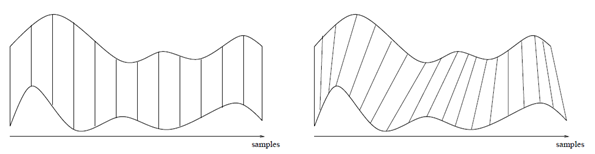
\includegraphics[width=1\textwidth]{./figures/dtw_dequence_demo}      
\caption{Sample-by-sample na\"{\i}ve alignment (left) versus an alignment performed using DTW (right) \cite{rath2003word}.}
\label{fig:dtw_dequence_demo}
\end{figure}

\iftoggle{edit-mode}{\hspace{0pt}\marginpar{Warping path Definition}}{}
\begin{definition}
Given two time series, $X = (x_1,x_2,...,x_n)$ and $Y = (y_1,y_2,...,y_m)$, the \emph{warping path} $W=(w_1,w_2,...,w_K)$ where ${w_k} = (i_k,j_k)$ is an alignment between the two sequences which satisfies the following conditions: 
\begin{enumerate}
\item Start and end point constraint: $w_1 = (1,1)$ and $w_k = (n,m)$. 
\item Local continuity constraint: ${w_{k + 1}} - {w_k} \in \left\{ {\left( {1,1} \right),\left( {1,0} \right),\left( {0,1} \right)} \right\}$
\end{enumerate}	 
The weight of a given warping path $W$ is defined as:
\begin{equation}
G(W) = \sum\limits_{k = 1}^{K} d(x_{i_k},y_{j_k} )
\end{equation}
where $d(x_{i_k},y_{j_k})$ is the distance between the points $x_{i_k}$ and $y_{j_k}$.
\label{def:warping_path}
\end{definition}

\iftoggle{edit-mode}{\hspace{0pt}\marginpar{DTW Definition}}{}
Equipped with the definition of a warping path, DTW is defined as follows:
\begin{equation}
DTW(X,Y)=\min\limits_{W} {G(W)}
\end{equation}
Namely, DTW returns the weight of the path which is associated with the optimal alignment.\\
Using a dynamic programming approach, DTW yields the optimal warping path by constructing the \emph{accumulated distance matrix} $D \in \mathds{R}^{m \times n}$. 
$D(i,j)$ is the minimum distance warping path that can be constructed from the two time series $X = \left( {{x_1},{x_2},...,{x_i}} \right)$ and $Y = \left( {{y_1},{y_2},...,{y_j}} \right)$.
The accumulated distance matrix is calculated as seen in Algorithm \ref{alg:adm_dtw}. \\
The value in $D(m,n)$ contains the minimum-distance warping path between $X$ and $Y$.
The optimal warping path $W$ is retrieved by backtracking the matrix $D$ from the point $D(m,n)$ to the point $D(1,1)$ following the greedy strategy of looking for the direction from which the current distance is taken \cite{senin2008dynamic}.
 
\begin{algorithm}
$D(1,1) = 0$\;
\For{$i\leftarrow 2$ \KwTo $n$}{
	$D(i,1) = d(x_i,y_1)$\;
}
\For{$i\leftarrow 2$ \KwTo $m$}{
	$D(1,j) = d(x_1,y_j)$\;
}
\For{$i\leftarrow 2$ \KwTo $n$}{
	\For{$j\leftarrow 2$ \KwTo $m$}{
		$D(i,j) = d(x_i,y_j) + \min {\left\{D(i,j - 1),D(i - 1,j),D(i - 1,j - 1)\right\}}$\;
	}
}
\caption{Accumulated distance matrix ($D$) construction}
\label{alg:adm_dtw}
\end{algorithm}

\iftoggle{edit-mode}{\hspace{0pt}\marginpar{stroke trajectories similarity measure using DTW}}{}
Handwritten strokes can be seen as temporal sequences in the planar space. 
In the on-line HWR, the exact temporal information is discarded in most cases by re-sampling the strokes to obtain equidistant sampling. 
However, unlike off-line HWR, the ordering information of the samples is kept. 
As such, DTW is an intuitive method for calculating the correspondence between two strokes. 
It have been proved to be relatively efficient and effective for shape matching of handwritten words. 
DTW was used in \cite{rath2003word, rath2003indexing, moghaddam2009application} to calculate the similarity between handwritten script in historical documents. 
Saabne has used DTW for key-word searching in \cite{saabni2011fast, saabni2008keyword}.


\iftoggle{edit-mode}{\hspace{0pt}\marginpar{DTW Speedup}}{}
The main drawback of DTW is its quadratic time and space complexity, i.e., $O(mn)$ where $m$ and $n$ are the time series lengths. 
Therefore, several speed-up methods have evolved \cite{salvador2007toward,rath2003word}.\textbf{Constraints enforcing}, i.e., limiting the amount of calculated cells in the accumulated distance matrix by imposing constrains on the calculation in the cells of the accumulated distance matrix, is a popular speed-up technique.
In some cases DTW tends to create an unrealistic correspondence between time-series features by aligning short features from one of the series to the long features on the second time series. 
To avoid this undesired phenomenon, constrains can be imposed on the possible correspondence between several consecutive points on the warping path. 
Two such constraints are the Sakoe-Chuba Band \cite{sakoe1978dynamic} and he Itakura parallelogram \cite{itakura1975minimum} as can be seen in Figure \ref{fig:dtw_dequence_demo}.
The greyed out area is the cells of the $D$ matrix that are filled by the DTW algorithm for each constraint. 
The warping path is looked for in the constraint window. 
The width of the window is specified by a parameter. 
Note that such constrains limit the amount of calculation needed for computing DTW, however, the speed-up factor is a constant and the DTW complexity remains quadratic. 
Furthermore, if the warping path is does not reside in the constraint window, it will not be found by DTW, therefore, such methods are usually used when the warping path is expected to be in the constrain window.


%\begin{compactitem}
%\item Constraints Enforcing: Limiting the amount of calculated cells in the accumulated distance matrix. 
%A more detailed explanation is given in the next paragraph.
%\item Data Abstraction: Speed-up using data abstraction is performed by running DTW on a reduced presentation of the data thus reducing the cell numbers that need to be computed. 
%The warp path is calculated on the reduced resolution matrix and mapped back to the original (full) cost matrix. 
%\emph{FastDTW} which was proposed in \cite{salvador2007toward} is an example of such approach.
%\item Lower Bounding: A lower-bounding is cheap and approximation of the DTW.
%It usually underestimates the actual cost determined by DTW. 
%It is used to avoid comparing series by DTW when the lower-bounding estimate indicates that the time series is worse match than the current best match \cite{rath2003word} 
%Lower bounding will be discussed in more details in Section \ref{subsec:lower_bounding}.
%\end{compactitem}

\iftoggle{edit-mode}{\hspace{0pt}\marginpar{How DTW is used in this work?}}{}
In this work, DTW is used for candidates re-scoring (described in chapter \ref{sec:candidates_scoring}). 
Actually, the $k$-NN are found among the entire dataset based on approximation of the EMD metric. 
Then, DTW is employed for attaching a more accurate similarity ranking between the query sample and its nearest neighbours.

\begin{figure}
\centering
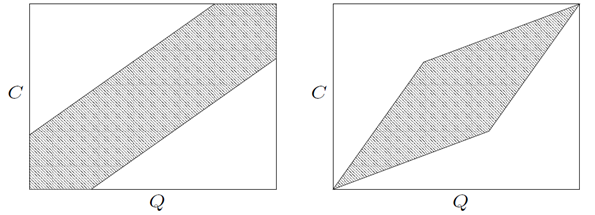
\includegraphics[width=0.7\textwidth]{./figures/dtw_sukoe_chuba}       
\caption{Cost matrix constraints: Sakoe-Chiba band (left) and the Itakura parallelogram (right).}
\label{fig:dtw_sukoe_chuba}
\end{figure}

%%%%%%%%%%%%%%%%%%%%%%%%%%%%%%%%%%%%%%%%%%%%%%%%%%%%%%%
\newpage{}
%%%%%%%%%%%%%%%%%%%%%%%%%%%%%%%%%%%%%%%%%%%%%%%%%%%%%%%

\section{Similarity Search}
\label{sec:similarity_search}
 
\iftoggle{edit-mode}{\hspace{0pt}\marginpar{Introduction}}{}
In Section \ref{sec:similarity_measures} we discussed the effectiveness aspect of measuring the perceptual notion of similarity between two objects.
However, even the most qualitative similarity measure technique is almost useless if for a given query object, the task of searching for similar objects in the database cannot be done efficiently.
Efficient similarity search usually requires the development of search methods that minimize the overall search costs.

\iftoggle{edit-mode}{\hspace{0pt}\marginpar{Similarity search query types}}{}
Similarity based search introduce two fundamental query types: \textbf{queries} and \textbf{k-NN queries} \cite{hetland2009basic}. 
Formal definitions of both query types are provided in Definitions \ref{def:range_query} and \ref{def:knn_query} and visualized in Figure \ref{fig:similarity_query_types}.
While range queries are argued to be fundamental, $k$-NN queries notably take a large volume in the literature.

\begin{definition}
Given a data space $\mathfrak{D}$, a distance function, $dist$, defined on $\mathfrak{D}$, a query object $q$ and a range parameter $r \geq 0$, the \textbf{range query} returns all the data objects in $\mathfrak{D}$ that are within distance $r$ from the query object $q$. 
Namely,
\begin{equation}
Range(q,r,\mathfrak{D},dist)=\{o \in \mathfrak{D} | dist(q,o) \leq r \}
\end{equation}
\label{def:range_query} 
\end{definition}

\begin{definition}
Given a data space $\mathfrak{D}$, a distance function, $dist$, defined on $\mathfrak{D}$, a query object $q$, the \textbf{k-nearest neighbours} (k-NN) query returns the $k$-closest objects in $\mathfrak{D}$ to the query object $q$. Formally,
\begin{equation}
k-NN(q,\mathfrak{D},dist)=\{A \subseteq \mathfrak{D} | \forall a \in A, b \in \mathfrak{D} \setminus A: dist(q,a) \leq dist(q,b) \wedge |A|=k \}
\end{equation}
\label{def:knn_query} 
\end{definition}

\begin{figure}[h!]
	\centering
        \fbox{\subfloat[]{
            \label{fig:range_query}
            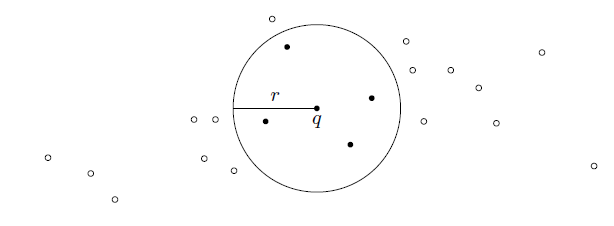
\includegraphics[width=0.4\textwidth]{./figures/range_query}
        }}
        \fbox{\subfloat[]{
           \label{fig:knn_query}
           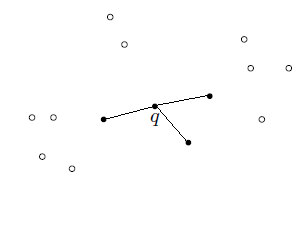
\includegraphics[width=0.4\textwidth]{./figures/knn_query}
        }}     
    \caption{Visualization of the \textbf{range} (\ref{fig:range_query}) and the \textbf{$k$-NN} (\ref{fig:knn_query}) queries in the two-dimensional Euclidean space.}
   \label{fig:similarity_query_types}
\end{figure}

\iftoggle{edit-mode}{\hspace{0pt}\marginpar{Problems - similarity search costs}}{}
The efficiency of a search method is defined as the time needed to evaluate a query. 
The query efficiency is affected mainly by two components; the \textbf{computation} cost and the \textbf{disk access time} (I/O) cost. 
The computation cost represents the effort spent in calculating the similarity measure function. 
The I/O cost is determined by the volume of data needed to be investigated to evaluate a query. Namely, the number of samples in the dataset that needs to be examined \cite{saabni2013efficient}.\\
Decreasing the computational cost can be obtained by using a cheap distance measure function which approximates, usually by providing a lower bound, the similarity between two given sample objects. 
The lower bound is used to filter out candidates with a similarity distance larger than a pre-set threshold. 
However, reducing the disk access cost can be attained only by discarding entire portions of the dataset which are assured to be distant enough from the given query object. 
Such techniques are called \emph{Metric Indexing} and will be discussed in Section \ref{sec:metric_indexing}.


\subsection{Lower Bounding}
\label{subsec:lower_bounding}
\iftoggle{edit-mode}{\hspace{0pt}\marginpar{Distance function approximation}}{}
In order to improve upon evaluating the distance function on every object in the dataset, we must somehow infer that an object $x$ can be included in, or excluded from, the search result without calculating the distance function $dist(q, x)$. One option to do so is by finding a cheap way of approximating the distance function. 
Although, both lower and upper bounding measures can be exploited to avoid running expensive calculation of the distance function $dist$, lower bounding appears to be more useful since it can be safely used to exclude far candidates, as described in Algorithm \ref{alg:lower_bound}. 
The more the approximation function $d$ is accurate, the less the actual distance function $dist$ will be invoked. However, there will normally be a trade-off between the approximation quality and the cost of computation \cite{hetland2009basic, keogh2005exact}.

\begin{algorithm}
$best\_so\_far = \infty$\;
\For{every object $x$ in database}{
	\If{$d(q,x) < best\_so\_far$}{
		$dist = d(q,x)$\;
	}
	\If{$dist < best\_so\_far$}{
		$best\_so\_far = dist$\;
		$nearest\_neighbor = x$\;
	}
}
\caption{A routine uses a lower bounding distance function, $d$, to speed-up the search for the nearest neighbour of the query object q in the database under the distance function $dist$.}
\label{alg:lower_bound}
\end{algorithm}

\subsection{Metric Embedding}
\label{subsec:metric_embedding}

\iftoggle{edit-mode}{\hspace{0pt}\marginpar{A different approach}}{}
The speed-up obtained by lower bounding is limited. 
An alternative approach is to embed the distance space imposed by the costly similarity measure, into a metric space equipped with a easy-to-compute distance function. 
Consequently, the calculation of distances between two elements in the embedded space would provide an inexpensive approximation to the actual distance between the two objects in the original space. 
A formal definition of the embedding is given in Definition \ref{def:embedding}.

\begin{definition}
Given metric spaces $(\mathfrak{D}, d)$ and $(\mathfrak{D}', d')$ a map $f : \mathfrak{D} \rightarrow \mathfrak{D}'$ is called an \textbf{embedding}.
\label{def:embedding}
\end{definition}

\iftoggle{edit-mode}{\hspace{0pt}\marginpar{Isometric embedding}}{}
The special case where $d(x, y) = d'(f(x), f(y))$ for all $x, y \in \mathfrak{D}$ is called \textbf{distance-preserving} or \textbf{isometric} embedding. However, isometric embeddings are very rarely beneficial, thus we allow the mapping to alter the distances in a restricted manner. The distortion of the embedding is defined in Definition \ref{def:embedding_distortion}.

\begin{definition}
Given two metrics $(\mathfrak{D}, d)$ and $(\mathfrak{D}',d')$ and a map $f : \mathfrak{D} \rightarrow \mathfrak{D}'$, the \textbf{contraction} of $f$ is the maximum factor by which distances are shrunk, i.e.,
\begin{equation}
\max_{x,y \in \mathfrak{D}} \frac{d(x,y)}{d'(f(x),f(y))}
\end{equation}
The \textbf{expansion} of $f$ is the maximum factor by which distances are stretched. Formally:
\begin{equation}
\max_{x,y \in \mathfrak{D}} \frac{d'(f(x),f(y))}{d(x,y)}
\end{equation}
and the \textbf{distortion} of $f$ is the product of the distortion and the expansion.
\label{def:embedding_distortion}
\end{definition}

\iftoggle{edit-mode}{\hspace{0pt}\marginpar{$L_p$ advantage and drawbacks}}{}
Using normed spaces (see Definitions \ref{def:norm}) such as the $L_p$ norm (see Definitions \ref{lp}) to solve the dissimilarity measure problem, allow using data structures that facilitate sub-linear $k$-NN retrieval.

\begin{definition}
Given a data space $\mathfrak{D}$, for any two data elements  $x,y \in \mathfrak{D}$, a \textbf{norm} $\|\cdot\|$ is defined as:
\begin{equation}
\|\cdot\|: \mathfrak{D} \longrightarrow \mathds{R}
\end{equation}
where the following conditions hold:
\begin{compactitem}
\item $\|x\|=0 \Leftrightarrow x=0$
\item $\|x-y\| \geq|\|x\|-\|y\||$
\item $\|\alpha x\|=|\alpha|\|x\|$
\end{compactitem}
the pair $\left(\mathfrak{D},\|\cdot\|\right)$ is called a \textbf{normed space}.
\label{def:norm}
\end{definition}


\begin{definition}
Given an vector space $V=\mathds{R}^N$ and $v=(v_1,v_2,...,v_N) \in V$, the $L_p$ norm is defined as:
\begin{equation}
\|v\|_p=\sqrt[p]{\sum\limits_{i=1}^N v_i^p}
\end{equation}
\label{lp}
\end{definition}
In this case we will denote this vector space as $L_p^N$ to emphasize the fact it is $N$ dimensional.

\subsection{Approximating EMD using Embedding}
\label{subsec:approximating_emd_using_embedding}

\iftoggle{edit-mode}{\hspace{0pt}\marginpar{Indyk and Thaper Embedding}}{}
Several approximation algorithms have been proposed to speed-up the computation of EMD. 
Indyk and Thaper \cite{indyk2003fast} proposed a technique for embedding the un-normed EMD metric into the $L_1$ space so that the EMD distance between the two objects is comparable to the Manhattan distance between the two points which represent the embedding of the two objects.  
Given two points sets $A$ and $B$, both of cardinality $N$ and containing points in $L_2^d$ space, the embedding given in \cite{indyk2003fast} is into the $L_1^d$ norm (i.e., the space of vectors in $\mathds{R}^d$ equipped with the Manhattan norm).
The general idea of the embedding is to compute and concatenate several weighted histograms of decreasing resolution for a given point set. 
Let us assume that the smallest distance between any two points is $1$, and $\Delta$ is the diameter of $C=A \bigcup B$. 
The embedding can be described as imposing hierarchy of grids $G_i$ having side length $2^i$ on the space $\mathds{R}^d$, where $-1 \leq i \leq \log \Delta$. 
It is required that each grid $G_{i}$ be a refinement of the grid $G_{i+1}$. 
Each grid is translated by a vector chosen randomly from $[0, \Delta]^d$. 
For each grid $G_i$, the vector $v_i(A)$ contains a single coordinate per cell that contains the number of points in the corresponding cell. 
In fact, for every $i$, $v_i(A)$ forms a histogram of A. 
The embedding, denoted as $f_{EMD}(A)$, is then defined as the concatenated vector of the $v_i$'s, scaled by the grid side lengths. 
Formally,
\begin{equation}
f_{EMD}(A) = [v_{-1}(A)/2, v_0(A), 2v_1(A), 4v_2(A),..., 2^iv_i(A),...]
\end{equation} 
Figure \ref{fig:emd_embedding} provides a visual demonstration of the embedding.
Approximating the EMD distance between the set $A$ and $B$ is then done by calculating the Manhattan distance between the two corresponding embedding vectors, i.e.,
\begin{equation}
EMD_{approx.}=|f_{EMD}(A) - f_{EMD}(B)|
\end{equation}  

\begin{figure}
\centering
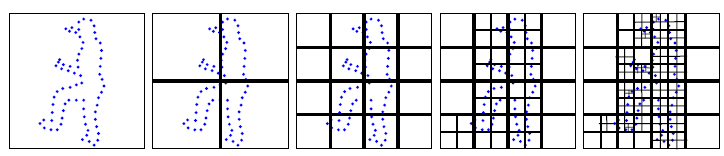
\includegraphics[width=0.7\textwidth]{./figures/emd_embedding}       
\caption{Embedding of a shape contour \cite{grauman2004fast}.}
\label{fig:emd_embedding}
\end{figure}

\iftoggle{edit-mode}{\hspace{0pt}\marginpar{Performance}}{} 
The time complexity of the embedding is $O(Nd \log{\Delta})$. 
The distortion of the embedding has an upper bound of $O(\log \Delta)$. 
A detailed proof is provided in \cite{indyk2003fast}. 
However, the proved theoretical distortion can only provide a weak practical instrument. 
Nevertheless, experimental validation performed on a dataset of $20,000$ objects showed a $(1+\epsilon)-approximate$ nearest neighbour, with $\epsilon < 20\%$ that was achieved by the embedding compared to the exact EMD. 
Grauman and Darrel \cite{grauman2004fast} have used this embedding for contour matching and experimentally validated the quality of retrieval. 
They have found that the accuracy reduction is less than $10\%$ compared to the exact EMD.

\subsubsection{EMD Embedding using the Wavelet Coefficients Domain}
%compare this embeddign technique to the previous one.
%How it is done?
%Is it faster to calculate?
%Is the retrieval more accurate (empirically) than the $L_1-EMD$ embedding?
%Are the bounds are more strict? 
%printf('%s','5ara 3leek ba7ebak') //by Reema Salma Darawshe

\iftoggle{edit-mode}{\hspace{0pt}\marginpar{Wavelet embedding}}{}
In a subsequent work done by Shirdhonkar and Jacobs \cite{shirdhonkar2008approximate}, the authors proposed a linear time method for approximating the EMD between two low dimensional histograms using the weighted wavelet coefficients of the difference histogram. 
It is done by calculating the $L_1$ norm of the coefficients vector of the embedding as given in Equation \ref{eq:emd_embedding}.

\begin{equation}
d(p)_{wemd}= \sum\limits_{\lambda} 2^{-j(1+n/2)}|p_{\lambda}|
\label{eq:emd_embedding}
\end{equation}
where $p$ is the n-dimensional difference histogram and $p_{\lambda}$ is the wavelet transform coefficients. 
The index $\lambda$ includes both shifts and the scale j.
They proved that the ratio of the approximation and the real EMD is bounded by constants. 

\iftoggle{edit-mode}{\hspace{0pt}\marginpar{Intuitive explanation}}{}
Intuitively, the wavelet transform splits up the difference histogram according to scale and location where each coefficient represents the solution to the EMD subproblem. 
For a single wavelet, the mass to be moved is proportional to the volume of $|\psi_j(x)|$, i.e., to $2^{-jn/2}$ and the distance to be travelled is proportional to the span of the wavelet, i.e $2^{-j}$. 
The sum of all distances is an approximation to EMD, as formally defined in Equation \ref{eq:emd_embedding}. 
This can be viewed similar to the way packages are shipped over large distances. 
The route is broken into several pieces which are large and small distances. 
Packages from nearby places are merged at the end of the short distance route piece to travel together. 
Then another merge is done of packages from the entire country to be shipped together to the destination country. 
The sum of the distances travelled is an approximation to the actual distance. 
See Figure \ref{fig:emd_wavelet}.

\begin{figure}
\centering
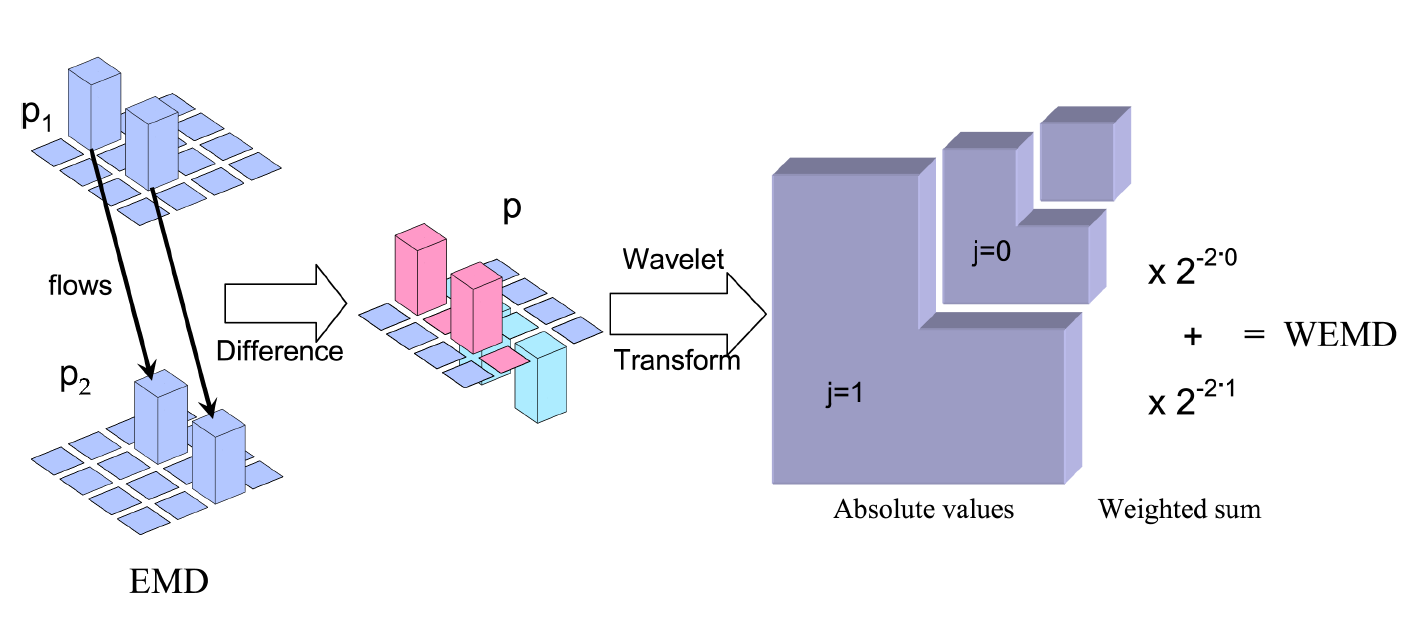
\includegraphics[width=1\textwidth]{./figures/emd_wavelet}       
\caption{EMD embedding using the wavelet domain \cite{shirdhonkar2008approximate}.}
\label{fig:emd_wavelet} 
\end{figure}

\iftoggle{edit-mode}{\hspace{0pt}\marginpar{Embedding the histograms rather than the difference histogram}}{}
However, in our application, where the histogram descriptors are to be stored rather than the difference histogram, the computation of EMD can be partitioned into two parts. 
First the histograms are converted into the wavelet domain and their coefficients are scaled according to Equation \ref{eq:emd_embedding}. 
Computing the EMD distance is done by calculating the Manhattan distance between the scaled coefficients of the corresponding histograms.

\iftoggle{edit-mode}{\hspace{0pt}\marginpar{shirdhonkar - theoretical and empirical bounds}}{}
Shirdhonkar and Jacobs provided both theoretical and experimental bounds. 
The theoretical approximation is based on Theorem 2 in \cite{shirdhonkar2008approximate}. 
Using a large dataset, they were able to experimentally establish that the proposed approximation follows the true EMD closely, and can be alternatively used without any significant difference in performance. 
The wavelet EMD metric can be computed in $O\left( N \right)$ time complexity. 

\iftoggle{edit-mode}{\hspace{0pt}\marginpar{Performance - Indyk vs. shirdhonkar}}{}
Empirically, the normalized RMS error obtained by using the wavelet embedding was between in 13\% and 20\% compared to the embedding proposed by Indyk and Thaper which achieved 43\% in the same experiment. 
In addition, the wavelet embedding surpassed the Indyk and Thaper embedding in time performance.
Note that the embedding process requires histograms, thus the vectors in the feature space need to be normalized before using this method.

Shirdhonkar and Jacobs tested few wavelets and showed that the \textbf{Coif-lets} of order 3 and the \textbf{Symmetric Daubechies} wavelets of order 5 have lowest error rates. 
We evaluated several wavelets, including the \textbf{Haar} wavelet, the \textbf{Coif-let} of order 1, the \textbf{Coif-let} of order 2 and the \textbf{Symlets} of order 5 wavelets.
The \textbf{Haar} wavelet achieved the best classification results.
Embedding the SC feature vectors has produces sparse vectors in $\mathds{R}^{2422}$.

 
%%%%%%%%%%%%%%%%%%%%%%%%%%%%%%%%%%%%%%%%%%%%%%%%%%%%%%%
\newpage{}
%%%%%%%%%%%%%%%%%%%%%%%%%%%%%%%%%%%%%%%%%%%%%%%%%%%%%%%

\section{Dimensionality Reduction}
\label{sec:dr}

\iftoggle{edit-mode}{\hspace{0pt}\marginpar{What is DR and what techniques are there?}}{}
\emph{Dimensionality Reduction} is a process of reducing the number of variables taken into consideration in the learning and classification of data. 
It is a fundamental process in machine learning since it facilitates classification, efficient storing and visualization of data. 
The undesired properties of high-dimensional data present many mathematical challenges and practical complications \cite{van2009dimensionality}. 
First, analysis of high-dimensional data generally requires a large amount of memory and computation power, which may be impractical for on-line classification systems and obstructive in other applications. 
In particular, several nearest neighbours retrieval methods such as $k$-d tree are ineffective when the dimensionality of the data is high.
Second, when the data dimensionality is high the classification algorithm is more likely to over-fit the training sample and generalizes poorly to new samples \cite{aida2009word}.
The high dimensional data phenomenon is widespread in data analysis and was given the name \emph{the curse of dimensionality}. 

\iftoggle{edit-mode}{\hspace{0pt}\marginpar{data Intrinsic dimensionality}}{}
Ideally, the dimensionality of the reduced representation should correspond to the intrinsic dimensionality of the data \cite{van2009dimensionality}.
The intrinsic dimensionality of data is the minimum number of properties needed to account for in the observed data. 
The belief underlying the existence of a compact representation of the external world data is based on the observation that the human brain can instantaneously and precisely recognize an observed apple, smile or a handwritten letter within a short route of neural computations. 
However, a digital representations of these images may consist of hundreds or thousands of pixels. 
Clearly, there are much more compact representations of images, sounds, and even text than their native digital formats. 
Several recently proposed dimensionality reduction techniques are based on the intuition that data lies on or near a complex low-dimensional manifold that is embedded in the high-dimensional space.

\iftoggle{edit-mode}{\hspace{0pt}\marginpar{The curse of dimensionality}}{}
The curse of dimensionality can arise in different stages of the learning and classification process; 1. the dimensionality of the raw data may be high, such as videos an images; 2. features calculated on the data may be impractically large; 3. other manipulations performed on the data may produce highly dimensional vectors.

\iftoggle{edit-mode}{\hspace{0pt}\marginpar{Why do we need DR?}}{}
The highly dimensional sparse vectors produced by the EMD embedding and the sensitivity of the $k$-d tree to high dimensional required us to add a dimensionality reduction stage.
The wish to employ $k$-d trees, which is very sensitive to high dimensional data, was the main reason for using dimensionality reduction. 
An alternative was to use a $k$-NN data-structure that performs well with high dimensional data such as \emph{Locality Sensitive Hashing} (LSH) \cite{gionis1999similarity}. 
However, it would be less accurate since LSH is an approximate NN search method, unlike $k$-d tree which can be used to find the exact $k$-NN samples.

\iftoggle{edit-mode}{\hspace{0pt}\marginpar{Mathematical Definition}}{}
Mathematically, given $p$-dimensional variable $x \in \mathds{R}^p$, the dimensionality reduction process finds a lower dimensional representation $s \in \mathds{R}^k$ with $k \ll p$ which preserves the content of the original data under a given criterion. 
The reduced dimensionality $k$ is chosen to be as small as possible, but yet sufficiently large to guarantee that the output vector $s$ provide a faithful representation of the input vector $x$. 
Dimensionality reduction techniques can be classified into linear and non-linear. \\
Linear dimensionality reduction is based on a linear projection of the data, assuming the data resides close to a lower dimensional linear subspace. 
Namely, each of the components in the vector $s$ is a linear combination of the components in the vector $x$, formally:
\begin{equation}
s=Wx
\end{equation}
where $W_{k \times p}$ is the linear transformation.

\iftoggle{edit-mode}{\hspace{0pt}\marginpar{Non-Linear DR}}{}
In some cases, linear dimensionality reduction techniques perform poorly and a intensified approach is required to provide the mapping from the high dimensional space to the low dimensional space. 
In such cases, non-linear techniques are used. 
Yet, the drawback of such techniques is concealed in its generality which may cause over-fitting on the sample set and not really capturing the true underlying coordinate system. 
Commonly used non-linear technique include \emph{Kernel PCA}, \emph{Isometric Feature Mapping} (ISOMAP) and \emph{Locally Linear Embedding} (LLE).

\iftoggle{edit-mode}{\hspace{0pt}\marginpar{What DR we use?}}{}
In this thesis we have chosen to work only with linear dimensionality reduction techniques. 
\emph{Principle Component Analysis} (PCA) and \emph{Linear Discriminant Analysis} (LDA) were applied sequentially in order to obtain linearly discriminative information efficiently.

\iftoggle{edit-mode}{\hspace{0pt}\marginpar{PCA}}{}
PCA is a popular linear dimensionality reduction technique proposed by Karl Pearson \cite{pearson1901principal} in 1901.
It is "unsupervised" in the sense that the labelling of the data do not effect the determination of the transformation function. 
PCA produces an orthogonal linear transformation that projects the data into a new coordinate system such that the greatest variance by any projection of the data comes to lie on the first coordinate (called the first principal component), the second greatest variance on the second coordinate (called the second principal component) and so on, as seen in Figure \ref{fig:pca_demo}. 
The principal components as a whole form an orthogonal basis. 
Given a multivariate dataset visualized as a set of coordinates in a high-dimensional data space, PCA obtains the "shadow" of that dataset when viewed from its most informative viewpoints by projecting the dataset into a lower-dimensional space formed by the first few principal components.

\begin{figure}
\centering
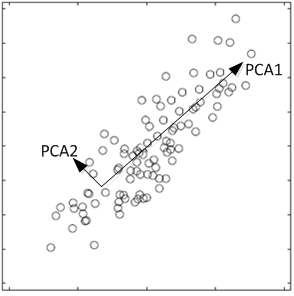
\includegraphics[width=0.4\textwidth]{./figures/pca_demo}       
\caption{The first and second principal component of the data elements, labelled as \emph{PCA1} and \emph{PCA2 }respectively.}
\label{fig:pca_demo}
\end{figure}

\iftoggle{edit-mode}{\hspace{0pt}\marginpar{PCA formulation}}{}
In computational terms the principal components are found by calculating the eigenvectors and eigenvalues of the data covariance matrix. 
This process is equivalent to finding the axis system in which the co-variance matrix is diagonal. 
The eigenvector with the largest eigenvalue is the direction of greatest variation. 
The eigenvalues represent the distribution of the source data energy among each of the eigenvectors, where the eigenvectors form a basis for the data. 
The representation content $g$ for the $j^{th}$ eigenvector is the sum of the energy content across all of the eigenvalues $\lambda_k$ from $1$ to $j$ :
\begin{equation}
g[j]=\sum_{k=1}^{j}\lambda_k 
\end{equation}
for $1 \leq j \leq d$ and $d$ denotes the dimensionality of the original data. 
The \emph{data preservation rate} value, $E$, is calculated as seen in Equation \ref{eq:dr_energy}. 
\begin{equation}
E[\ell] = \frac{g[\ell]}{g[d]}
\label{eq:dr_energy} 
\end{equation} 
The goal is to find the smallest possible $\ell$ that achieves $E[\ell]$ value which rise above a pre-set threshold, usually larger than $0.9$. 
This dimensionality estimation technique is known as the \emph{eigenvalue-based dimensionality estimator}. 

\iftoggle{edit-mode}{\hspace{0pt}\marginpar{LDA}}{}
The major drawback of PCA is that it is an unsupervised technique and as such does not use label information of the data. 
The following example, given by Welling in \cite{welling2005fisher}, demonstrates the problem in using PCA. 
In Figure \ref{fig:cigarettes_data}, we see two parallel cigar like clusters. 
The variance of the entire sample set, disregarding the labels, is in the direction of the cigars. 
Projecting the sample set on the principal component would terribly mix the samples. 
Clearly, a better projection would be orthogonal to the cigars, namely in the direction of least overall variance, which perfectly separate the two classes.
LDA, a descendant of the original Fisher-LDA \cite{fisher1936use}, overcomes this problem. 
Unlike PCA, LDA is a supervised technique. 
It attempts to model the difference between classes of data based on the samples labelling. 
In this method, variability among the feature vectors of the same class is minimized and the variability among the feature vectors of different classes is maximized. 
LDA performs dimensionality reduction while preserving as much of the class discriminatory information as possible. 
A brief tutorial on LDA is given in \cite{balakrishnama1998linear}. 
Without going into the math, in order to find a good projection vector, we need to define a measure of separation between the projections. 
The solution proposed by Fisher is to maximize a function that represents the difference between the means, normalized by a measure of the within-class scatter. 
LDA has three main drawbacks; the first is that it assumes that the data resides in $L_2$; second, LDA assumes that the distribution of the samples in each class is Gaussian which is not necessarily true; third, it is much slower to calculate compared to PCA.
Note that even though LDA is preferred in many application, it does not always outperform PCA.  


\begin{figure}
	\centering
        \subfloat[]{
            \label{fig:ldapca}
            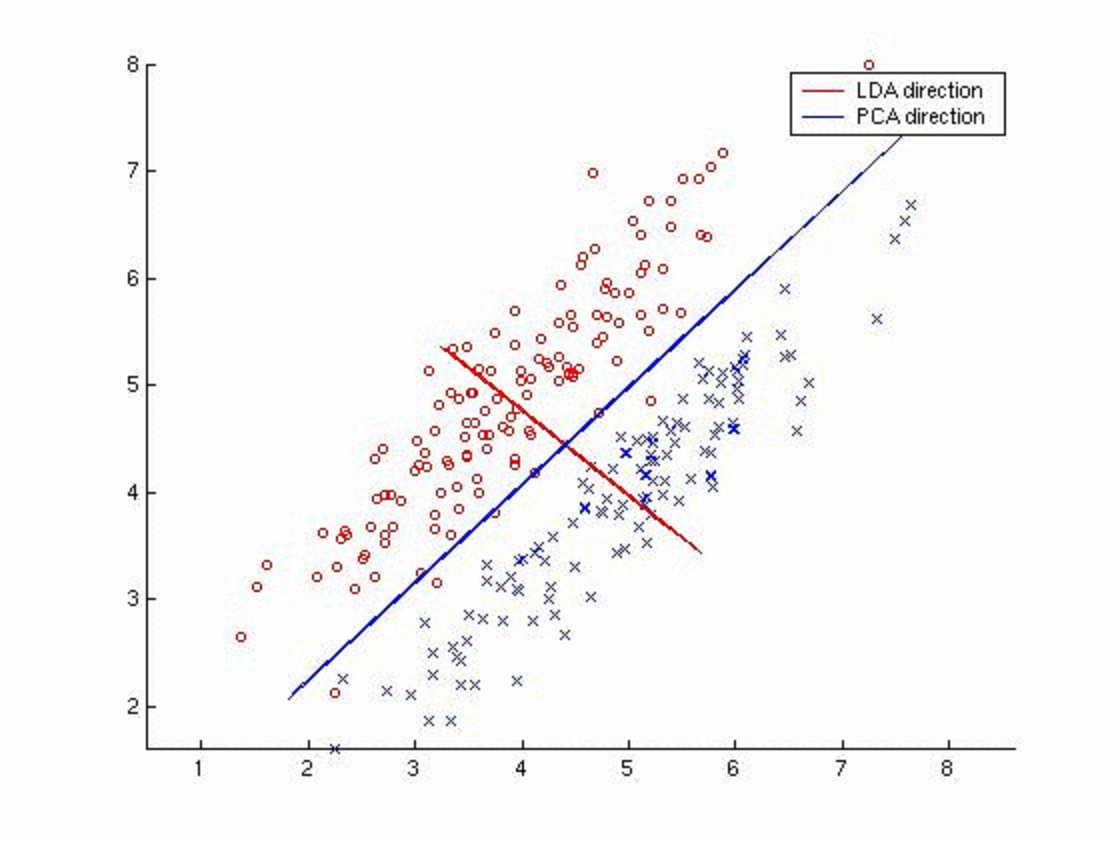
\includegraphics[width=0.5\textwidth]{./figures/ldapca}
        }
        \subfloat[]{
           \label{fig:ldapca_graph}
           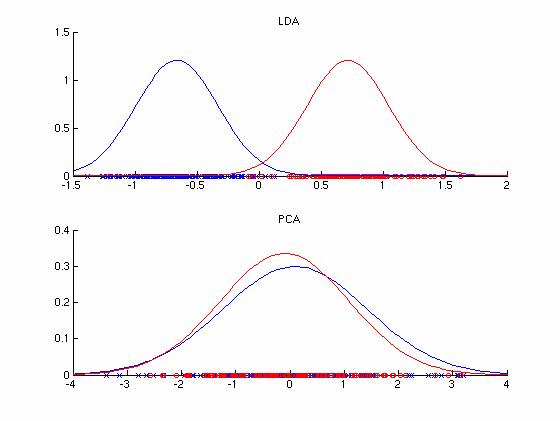
\includegraphics[width=0.5\textwidth]{./figures/ldapca_graph}
        }
    \caption{A cigarettes like spread of data samples is shown in \ref{fig:ldapca}. 
    The samples projection and distribution in the PCA and LDA projection directions is compared in \ref{fig:ldapca}}
   \label{fig:cigarettes_data}
\end{figure}


\iftoggle{edit-mode}{\hspace{0pt}\marginpar{When to perform the DR?}}{}
Grauman et al. in \cite{grauman2004fast} used PCA to find a low-dimensional subspace based on a large sample of the SC histogram. 
PCA yields the set of bases that define a low-dimensional "shape context manifold". 
Only then the approximate EMD embedding is performed. 
However, we have chosen to perform the stages in a different order. 
First, approximate EMD embedding is performed on the feature vectors, and only then, dimensionality reduction procedure is applied on the sparse embedded vectors. 
The reason we have chosen to perform the stages in this order is that if we were to apply the order suggested by Grauman, we would still result in a large sparse vectors constructed by the embedding process.
  
\iftoggle{edit-mode}{\hspace{0pt}\marginpar{Usage of PCA in the $L_1$ space.}}{}
PCA and LDA are basically defined over $L_2$ while the embedding into the wavelet coefficients domain was proved to approximate EMD in $L_1$. 
Nevertheless, we decided to use the basic form of PCA, given that $L_2$ estimates $L_1$ fairly well.

\iftoggle{edit-mode}{\hspace{0pt}\marginpar{Implementation: PCA}}{}
In order to exploit the strengthens of both PCA (efficiency) and LDA (discrimination power) we've used the dimensionality reduction process outlined as follows. 
The data samples are projected to a subspace $S_1$ using PCA and then to subspace $S_2$ using LDA. 
In the PCA stage, the target dimensionality, is the minimal to achieve data preservation rate of 99\%. 
As mentioned before, the dimensionality of the embedded vectors was $2422$. 
The reason we adopted such high preservation rate is that it was enough to secure a major dimensionality reduction. 
As seen in table \ref{table:dr_dimensions_results}, the dimensionality was reduced in two orders of magnitude by PCA.

\begin{table}
\centering
\caption{The dimensionality of the four datasets after applying PCA and PCA+LDA.}
\begin{tabular}{ c c c c }
\toprule
\textbf{Letter position} & \textbf{Number of samples} & \textbf{PCA} & \textbf{PCA+LDA} \\
\midrule                 
  Ini & 1405 & 48 & 9 \\ 
  Mid & 1196 & 52 & 10 \\ 
  Fin & 1629 & 44 & 9 \\ 
  Iso & 1372 & 39 & 8 \\ 
  \bottomrule
\end{tabular}
\label{table:dr_dimensions_results} 
\end{table}

\iftoggle{edit-mode}{\hspace{0pt}\marginpar{Implementation: Clustering and LDA}}{}
Applying LDA directly on the resulted data would have achieved poorer results due to the fact that almost all letters in the Arabic writing system have several shapes, relatively different, which are commonly used. 
Since LDA regards the labelling of the data samples, trying to group different perceptual shapes in a single class would impinge the dimensionality reduction process. 
In order to overcome this obstacle, we have done the following preprocessing steps: each class, namely the tuple $(letter, position)$, was clustered into four clusters using $L_1$-k-medoids algorithm. 
Each cluster received a unique class label. 
This new artificially labelled data was given as input to the LDA.

\iftoggle{edit-mode}{\hspace{0pt}\marginpar{LDA target dimensionality}}{}
Determining the target dimensionality of the LDA stage was done using the \emph{Maximum Likelihood Estimation} (MLE) method described in \cite{levina2004maximum}.
MLE belongs to a family of dimensionality estimation methods called \emph{Intrinsic dimensionality estimation}.
Intrinsic dimensionality estimation techniques are based on the observation that for a given data point $x_i$ the number of sample points covered by a hypersphere around the data point with radius $r$ grows proportional to $r^d$; where $d$ is the intrinsic dimensionality of the data manifold around that data sample.  
The function that estimates this relation for a given data point $x_i$ is named \emph{local estimator}.
The estimated intrinsic dimensionality $\hat{d}$ of the dataset is then calculated by averaging over the local estimators of the entire sample set \cite{van2007introduction}.

\iftoggle{edit-mode}{\hspace{0pt}\marginpar{The DR package}}{}
The dimensionality reduction stage was implemented using the \textbf{Matlab Toolbox for Dimensionality Reduction} package described in \cite{van2007introduction}.

%%%%%%%%%%%%%%%%%%%%%%%%%%%%%%%%%%%%%%%%%%%%%%%%%%%%%%%
\newpage{}
%%%%%%%%%%%%%%%%%%%%%%%%%%%%%%%%%%%%%%%%%%%%%%%%%%%%%%%


\section{Metric Indexing}
\label{sec:metric_indexing}

\iftoggle{edit-mode}{\hspace{0pt}\marginpar{Motivation}}{}
Distance function approximation techniques alone cannot avoid linear scan of the entire dataset when searching for the $k$-NN of a query object. 
Efficient data retrieval in a metric dataset requires building a \emph{metric index}.
The main goal of indexing methods is to enable efficient searching, either asymptotically or simply in real wall-clock time. 
The time cost involved in building the index is amortized over the series of queries, and is usually ignored when considering search cost, and the fact that in most cases it is an off-line process \cite{hetland2009basic}.

\iftoggle{edit-mode}{\hspace{0pt}\marginpar{Introduction}}{}
Indexing techniques partition the dataset into equivalence classes in a way that each equivalence class contains objects that are sufficiently close to each other. 
However, this does not assure that close objects will always be contained in the same equivalence class. 
Each class is bounded by a hypersphere covering all the objects in the equivalence class. Consequently, at query time the index is efficiently searched to locate the equivalence classes which cover the areas where the closest objects may be contained. 
These classes are then exhaustively checked for the relevant objects.
This allows discarding classes that surely does not contain relevant objects. 
In order for the metric indexing to work correctly and efficiently, the distance function is required to satisfy the triangle equality.
 
\iftoggle{edit-mode}{\hspace{0pt}\marginpar{Exact vs. Approximate Indexing}}{}
Metric indexing techniques are split into two types: exact and approximate. 
Exact techniques are guaranteed to return the same result as  scanning the entire database. 
Approximate indexing methods return good matches, but not necessarily the best matches. 
Exact methods do not allow false positives or false negatives, i.e., all of the relevant objects are required to be returned in the query result, and only them. 
However, the approximate methods relax this strong requirement so that a small number of false negatives is acceptable \cite{keogh2005exact}. 
Many methods were proposed to solve the exact $k$-NN problem that are significantly better than a brute-force computation over the entire database. 
However, computing the approximate nearest neighbours, can achieve significantly faster retrieval with a relatively small actual error. 
Approximate nearest neighbours techniques also allow the user to specify a maximum approximation error bound, thus enabling the user to control the trade-off between accuracy and running time.

\begin{figure}
\centering
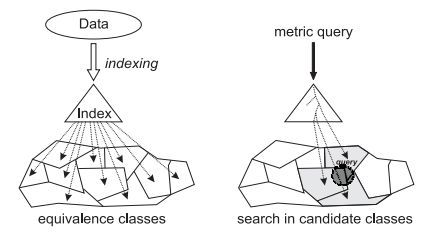
\includegraphics[width=0.7\textwidth]{./figures/indexing}       
\caption{Metric indexing and query.}
\label{fig:indexing}
\end{figure}

\iftoggle{edit-mode}{\hspace{0pt}\marginpar{Examples of Exact and Approximate Indexing}}{}
Approximate nearest neighbours methods such as $k$-d trees and LSH have been successfully applied on a variety of fast similarity retrieval problems.
The key assumption in these procedures is that the objects in the dataset lie in a metric space, i.e., the space satisfies the triangle equality; an assumption which may not be valid for many similarity measure techniques.
The $k$-d tree even requires a stronger requirement of $L_p$ space. 

\iftoggle{edit-mode}{\hspace{0pt}\marginpar{This work}}{}
While the advantage of LSH is that it performs better than $k$-d tree in high dimensional spaces, $k$-d tree can be used both as an exact and approximate $k$-NN technique. 
In this work, we have chosen to work with $k$-d tree since we could obtain, after applying the dimensionality reduction stage, a low dimensional data space.
In addition, the sensitivity of the segmentation process requires high classification accuracy.

%%%%%%%%%%%%%%%%%%%%%%%%%%%%%%%%%%%%%%%%%%%%%%%%%%%%%%%
\subsubsection{$k$-d tree}

\iftoggle{edit-mode}{\hspace{0pt}\hspace{0pt}\marginpar{A short introduction to $k$-d tree}}{} 
The $k$-d tree is an efficient data structure for storing a finite set of points from a $k$-dimensional space, proposed by Bentley in \cite{bentley1975multidimensional}. 
It aims at solving the $k$-NN problem in a large set of multi-dimensional points by first building a data structure based on the set of reference points. 

\iftoggle{edit-mode}{\hspace{0pt}\marginpar{How it works, how the data is saved and extracted}}{} 
The $k$-d tree is constructed as follows. 
Every point is either a branch node or contained in a leaf node. 
Every branch node in the tree is associated with one of the $k$-dimensions and can be though of an hyperplane that divides the space into two half spaces in that dimension. 
Points to the left of this hyperplane are represented by the left sub-tree of that node and points to the right of the hyperplane are represented by the right sub-tree, see Figure \ref{fig:kd_tree}. 
A desired property of the partition is to be as equal as possible. 
The selection of the pivot point (i.e,  the point that function as a branch node) in every level has a great impact on the balance of the tree. 
The most common way is to find the medial point of a number of points in the sub-tree. 
The number of points in a leaf node is also customizable and is mostly affected by the cardinality of the points in the database and the typical $k$, which is a predefined in many applications.

\begin{figure}
\centering
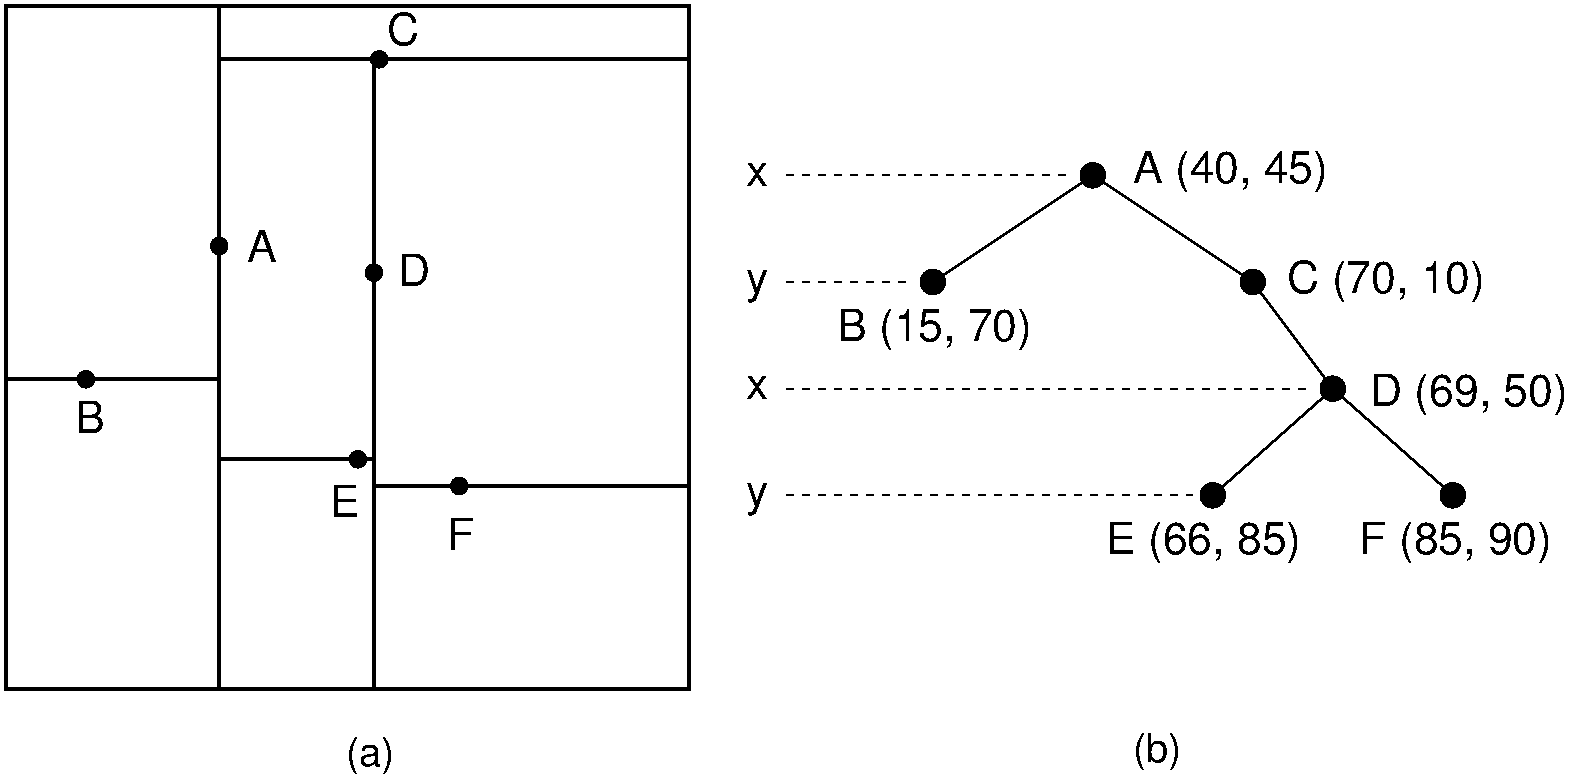
\includegraphics[width=0.8\textwidth]{./figures/kd_tree}       
\caption{Example of a $k$-d tree. (a) - The $k$-d tree decomposition of a region containing six data points. (b) - The $k$-d tree representation for (a).}
\label{fig:kd_tree}
\end{figure}

\iftoggle{edit-mode}{\hspace{0pt}\marginpar{How the NN are found?}}{}
The approximation of the $k$-NN in a $k$-d tree is done by initially finding the leaf node that represents the equivalence class that the query point belongs to. 
Although it is probable that the $k$-NN are all contained in a single leaf node, it is not necessarily the case. 
Adjacent leafs may be examined by recursively explore the other child nodes and look for the exact $k$-NN. 
 
\iftoggle{edit-mode}{\hspace{0pt}\marginpar{Expected time complexity}}{}
The construction time of the $k$-d tree is O($k N \log N$), where $k$ is the dimensionality of the data space and $N$ is the cardinality of the dataset. 
We can afford this high complexity of the construction since the this process is done off-line, and theoretically will be executed mostly several times. 
Therefore, this tax pays off when it comes to the enhancement we achieve in the k-$NN$ query evaluation. 
While the worst case scenario, the running time of $k$-NN is $O(N^{d^2})$, the amortized running time is $O(\log N)$.

\iftoggle{edit-mode}{\hspace{0pt}\marginpar{The Matlab library}}{} 
Our system uses a built-in Matlab implementation for $k$-d tree which is available in the statistical toolbox and introduced in Matlab R2013B. 
The library allows configuring the distance function (Euclidean, Manhattan, Mankowski, etc...) and the size of the leaf node. 
The library provides an implementation for the exact version of $k$-d tree.

%%%%%%%%%%%%%%%%%%%%%%%%%%%%%%%%%%%%%%%%%%%%%%%%%%%%%%%
\newpage{}
%%%%%%%%%%%%%%%%%%%%%%%%%%%%%%%%%%%%%%%%%%%%%%%%%%%%%%%

\section{Candidates Re-scoring}
\label{sec:candidates_scoring}
\iftoggle{edit-mode}{\hspace{0pt}\marginpar{The need for a re-scoring}}{} 
Given an unlabelled sequence $q$, the $k$-NN classifier, using the Manhattan distance, returns a set of $k$ potential letter candidates from the sample set and their scoring, i.e., the perceptual distance between the candidate and $q$.
As mentioned in Section \ref{def:embedding}, the Manhattan distance in the wavelets coefficients domain approximate the EMD distance between objects. 
However, in implementations that require exact scoring of the candidates, the approximated EMD distance may not be sufficient and an additional scoring stage should be employed to obtain a more accurate similarity measure between the query object and the candidates.
Nevertheless, as explained in Section \ref{sec:similarity_measures}, in most cases such similarity measure techniques are computationally expensive and can be applied only on a short list of candidates rather than on the entire sample set.   

\iftoggle{edit-mode}{\hspace{0pt}\marginpar{How re-scoring is done here}}{} 
In this work, re-scoring of the candidates is done by calculating the DTW distance between the preprocessed version of the query sequence and the candidates.
The constrained version of DTW using the Sakoe-Chuba Band \cite{sakoe1978dynamic} demonstrated better results than the unconstrained version of DTW.
$k$, the number of candidates returned by the $k$-d tree, is set to 10.
As we will see in the results sections, the re-scoring stage significantly affects the classification performance, in terms of accuracy and response time.\\
In order to measure the re-scoring effectiveness, in Section \ref{sec:classification_results} we compare between the classifier results when including and when avoiding the re-scoring stage.

%%%%%%%%%%%%%%%%%%%%%%%%%%%%%%%%%%%%%%%%%%%%%%%%%%%%%%%
\newpage{}
%%%%%%%%%%%%%%%%%%%%%%%%%%%%%%%%%%%%%%%%%%%%%%%%%%%%%%%

\section{Experimental Results}
\label{sec:classification_results}

\subsection{Classification Quality Measures}
\iftoggle{edit-mode}{\hspace{0pt}\marginpar{Classification types}}{}
There are three commonly used classification quality measurements for assessing the performance of a classification algorithm: \emph{Accuracy}, \emph{Precision} and \emph{Recall}.
In binary classification, each sample belongs to one of two classes, the positive class or the negative class.
A \emph{true positive} ($tp$) instance is an actual positive sample classified correctly as positive by the classification system.
Similarly, a \emph{true negative} ($tn$) instance is the case of a negative sample classified correctly as negative.  
Wrong classification of samples are of two types: a positive sample mistakenly classified as negative, named \emph{false positive} ($fp$), and the case of a negative sample classified as belonging to the positive class, i.e.,  \emph{false negative} ($fn$). 

\iftoggle{edit-mode}{\hspace{0pt}\marginpar{Classification quality measurements - binary}}{}
The \emph{Accuracy} is the fraction of the points in the sample set that were classified correctly. 
Formally,
\begin{equation}
\text{Accuracy}=\frac{tp+tn}{tp+fp+tn+fn}
\label{eq:accuracy}
\end{equation}
\emph{Precision} is the fraction of true positive among all the instances classified as positive. Namely,
\begin{equation}
\text{Precision}=\frac{tp}{tp+fp}
\label{eq:precision}
\end{equation}
The measure \emph{Recall} is the fraction of instances correctly classified as positive among all the positive samples, calculated as described in Equation \ref{eq:recall}.
\begin{equation}
\text{Recall}=\frac{tp}{tp+fn}  
\label{eq:recall}
\end{equation}
Precision can be seen as a measure of exactness or quality, whereas recall is a measure of completeness.

\iftoggle{edit-mode}{\hspace{0pt}\marginpar{Classification quality measurements - multi-class}}{}
The classification quality measures in multi-class classification problems are the generalization of the binary class quality measures.
The \emph{confusion matrix} built from the classifier results allows visualization of the classifier's performance \cite{sokolova2009systematic, labatut2012accuracy}. 
Given a $k$-class classification problem and a sample set containing $n$ instances, let us denote the true classes as $C_i$ whereas the estimated classes, returned by the classifier, to be denoted as $\hat{C}_i$ for $i\leq i \leq k$.
In the confusion matrix, seen in Equation \ref{eq:confusion_matrix}, $n_{ij}$ corresponds to the number of instances belongs to class $j$ and classified as belongs to class $i$.

\begin{equation}
\bordermatrix{ & C_1& \ldots &C_k \cr 
  \hat{C}_i & n_{11} & \cdots & n_{1k} \cr
  \vdots    & \vdots & \ddots & \vdots \cr
  \hat{C}_k & n_{k1} & \cdots & n_{kk}}
\label{eq:confusion_matrix} 
\end{equation}
The corresponding overall accuracy, precision and recall measures in the multi-class case are calculated based on the confusion matrix as follows:
\begin{equation}
\text{Accuracy}=\frac{\sum\limits_{i=1}^{k} n_{ii}}{n}
\label{eq:k_accuracy}
\end{equation}

\begin{equation}
\text{Precision}=\frac{\sum\limits_{i=1}^{k} \frac{n_{ii}}{\sum_{j=1}^{k} n_{ji}}}{k}
\label{eq:k_precision}
\end{equation}

\begin{equation}
\text{Recall}=   \frac{\sum\limits_{i=1}^{k} \frac{n_{ii}}{\sum_{j=1}^{k} n_{ij}}}{k}
\label{eq:k_recall}
\end{equation}

\subsection{The Characters Classifier Performance}
\iftoggle{edit-mode}{\hspace{0pt}\marginpar{The sample set}}{}
The characters sample set contains 1404 samples of \textbf{Initial} letters, 1195 \textbf{Medial} letters, 1628 \textbf{Final} samples and 1371 \textbf{isolated} letter samples.
As previously mentioned, the classifier contains four databases, one for each position. 
It receives a sequence of points $S=\{p_{i}\}_{i=1}^{n}$ representing the letter trajectory and a letter position $\phi \in \{Ini, Mid, Fin, Iso\}$, and returns the classification of the sample in that corresponding database.
Below, we give a detailed evaluation of the classifier performance in terms of accuracy and running time.

The accuracy and the time performance of the classifier was measured using 10-fold cross-validation.
In Table \ref{table:results_position}, the accuracy, recall and precision rates are given for each character position dataset.
The last row in Table \ref{table:results_position} shows the accumulative average of the results weighted according to the amount of samples in each dataset.

\begin{table}
\centering
\caption{Characters classification results.}
\renewcommand{\arraystretch}{1.2}
\begin{tabular}{c c c c c}
\toprule
	\textbf{Character Position} & \textbf{Accuracy} & \textbf{Recall} &  \textbf{Precision} \\
	\midrule
	Ini & 93\% & 85\% & 88\% \\                
  	Mid & 89\% & 87\% & 90\% \\
  	Fin & 91\% &  86\% & 92\% \\
  	Iso & 91\% &  81\% & 90\% \\
  	\midrule
  	\textbf{Overall} & \textbf{91\%} &  \textbf{85\%} & \textbf{90\%} \\
  	\bottomrule
\end{tabular}
\label{table:results_position} 
\end{table}

In Table \ref{table:configurations} we propose several activation configurations of the presented classifier that target different balance points between accuracy and time performance.
In each experiment, the classifier performance was measured in terms of accuracy and the average response time for classifying a single sample.

In the first configuration, titled \textbf{\emph{High Accuracy}}, we evaluate the classifier as presented in this work, including the re-scoring stage described in Section \ref{sec:candidates_scoring}.
This configuration should be used in implementations which require high classification rate and can tolerate a certain degree of latency.

In the second configuration, named \textbf{\emph{Low Latency}}, the re-scoring stage is skipped.
As can be seen in Table \ref{table:configurations}, the response time in this configuration is significantly lower compared to the first configuration.
Applying the re-scoring stage, although being invoked on a short list of candidates, has a considerable impact on the classifier time performance. 
This configuration should be considered in cases where the time performance is a critical factor, such as in real-time classification and recognition-based script segmentation systems.
When the top three candidates are considered, the difference in accuracy is small between the first and second configurations, and the latency resulted from the re-scoring process done in the first configuration, in most cases, will not pay. 

The dimensionality reduction and the indexing processes are both computationally expensive and time consuming. 
Although both stages are usually performed off-line in the learning stage, in systems in which the learning is performed on-line, the latency they impose on the learning process is undesired.
Thus, in the third configuration, named \textbf{\emph{Fast Learning}}, both the dimensionality reduction and the indexing stages were omitted from the learning process.
In addition, no re-scoring is performed in the classification flow.
Comparing the results of the this configuration with the second configuration shows that the dimensionality reduction process done in the second configuration has improved the time performance of the classifier significantly, without affecting much the classification rate.
We have noted that the vast majority of the delay in the learning process was caused by the dimensionality reduction stage rather than from the indexing process.
However, due to the sensitivity of the $k$-d tree to high dimensional data, when omitting the dimensionality reduction process, one should not perform indexing using $k$-d tree because it would negatively affect the classification repose time.

\begin{table}
\centering
\caption{Classification accuracy and time performance of three activation configurations.}
\renewcommand{\arraystretch}{1.2}
\begin{tabular}{ c c c c }
  \toprule
  \textbf{Configuration}  & \textbf{Accuracy [Top 1]}  & \textbf{Accuracy [Top 3]} & \textbf{Time [ms]}\\
  \midrule
  High Accuracy & 91\% & 96\% & 29.9 \\ 
  Low Latency   & 87\% & 94\% & 0.12 \\
  Fast Learning & 90\% & 96\% & 4.4 \\ 
  \bottomrule
\end{tabular}
\label{table:configurations} 
\end{table}

Tables \ref{table:results_position} and \ref{table:configurations} show the results of experiments performed using the SC as the shape descriptor.
Table \ref{table:features_comparison} compares the performance of the the MAD and the SC descriptors by running the classifier in the \textbf{\emph{High Accuracy}} configuration using each descriptor.
One possible reason the SC achieved higher classification rate that the MAD is that vectors produced by the SC, in our implementation, has the same overall mass and thus the EMD is a metric, unlike the feature vectors produced by the MAD.

\begin{table}
\centering
\caption{Comparing the accuracy rates of the different feature extraction techniques.}
\renewcommand{\arraystretch}{1.2}
\begin{tabular}{ c c c }
    \toprule
	\textbf{Shape Descriptor}  & \textbf{Accuracy [Top 1]}  & \textbf{Accuracy [Top 3]} \\
	\midrule 
	SC      & 91\% & 96\%  \\                
  	MAD     & 88\% & 94\% \\
  	None    & 87\% & 93\% \\
  	\bottomrule
\end{tabular}
\label{table:features_comparison} 
\end{table}

%\bibliographystyle{plainnat}
%\bibliography{references}
%\end{document}
